\documentclass[bulk=0.052mm]{cover}% G-Print 115, PUR
\usetikzlibrary{fadings}
\def\thesistitle{Programming Models for Many-Core Architectures}
\def\thesissubtitle{A \Codesign Approach} % can't decide on co-design or codesign yet...
\def\thesisauthor{Jochem~H.\ Rutgers}
\def\thesisauthorinitials{JHR} % mainly used for prefixing \cite{}s to self
\def\thesisdate{2014-05-14} % date of defense, must be in ISO 8601
\def\thesistime{14:45} % time of defense, probably one of 12:45, 14:45, and 16:45

\def\thesisISBN{978-90-365-3611-0}
\def\thesisDOI{10.3990/1.9789036536110}
\def\thesisISSN{1381-3617}
\def\thesisCTITnr{14-292}

\title{\thesistitle}
\author{\thesisauthor}

		\tikzfading[name=invitation fade,top color=transparent!10,bottom color=transparent!100]
\begin{document}
\def\normalfont{\color{white}\sffamily\lsstyle}

\definecolor{text back color}{hsb}{0.66,0.35,0.24}

\tikzset{
	cover font/.style={outer sep=0,inner sep=2ex,font=\normalfont},
%
	title/.style =		{cover font,inner xsep=0,anchor=center},
	subtitle/.style =	{cover font,inner xsep=0,anchor=center},
	author/.style =		{cover font,inner xsep=0,anchor=center},
	spine text/.style =	{cover font,inner xsep=0,anchor=mid,rotate=-90},
	invitation text/.style={cover font,anchor=north,inner xsep=1cm,inner ysep=1.5ex},
%
	shadow/.style={contour=black!80},
	text back/.style={fill=text back color,opacity=.5,outer sep=0,inner sep=0,rounded corners=1mm},
	isbn/.style={fill=white},
}

\def\covertext[#1] (#2) at (#3) #4#5@#6;{
	\begin{pgfonlayer}{foreground}\normalfont#6\node[#1,font=#6] (#2) at (#3) {\parbox[c]{#4}{\strut#5\strut}};\end{pgfonlayer}
	\begin{pgfonlayer}{shadow}\normalfont#6\node[#1,shadow,font=#6,anchor=north west] (#2 shadow) at (#2.north west) {\parbox[c]{#4}{\strut#5\strut}};\end{pgfonlayer}
}

%%%%%%%%%%%%%%%%%%%%%%%%%%%%%%%%%%%%%
%% Background

\begin{scope}
	\path[clip] ($(back cover.north west)+(-\bleedwidth,\bleedwidth)$) rectangle ($(front cover.south east)+(\bleedwidth,-\bleedwidth)$);
	\def\dobackgroundimg{\node[anchor=center,inner sep=0,outer sep=0] at (center) {\imgRs[55]{cover}{jpg}{\coverwidth+1.8\bleedwidth}};}
	\iflowres
		\iffrontonly
			\def\dobackgroundimg{\node[anchor=west,inner sep=0,outer sep=0] at (center) {\imgRs[150]{cover}{jpg}[+repage -gravity East -crop 50\%x100\%]{.5\coverwidth+0.9\bleedwidth}};}
		\fi
		\ifbackonly
			\def\dobackgroundimg{\node[anchor=east,inner sep=0,outer sep=0] at (center) {\imgRs[150]{cover}{jpg}[+repage -gravity West -crop 50\%x100\%]{.5\coverwidth+0.9\bleedwidth}};}
		\fi
	\fi
	\dobackgroundimg
\end{scope}

%%%%%%%%%%%%%%%%%%%%%%%%%%%%%%%%%%%%%
%% Spine

\begin{coverspine}
	\SetTracking[spacing={300*,,}]{encoding=*}{10}
	\covertext[spine text] (author) at ($(spine.north)!.5!(spine.south)$) {.9\spineheight}{\thefulltitle\hfill\thesisauthor}@\Large;
	\node[text back,fit={(spine)},inner xsep=0,inner ysep=.5cm,outer sep=0,rounded corners=0] {};
\end{coverspine}
	
%%%%%%%%%%%%%%%%%%%%%%%%%%%%%%%%%%%%%
%% Back cover

\begin{coverback}
	\node[isbn,outer sep=1cm,anchor=south west] (isbn) at (back cover.south west) {\edef\args{[SC0,ISBN=\thesisISBN]}\expandafter\EANisbn\args};
\end{coverback}

%%%%%%%%%%%%%%%%%%%%%%%%%%%%%%%%%%%%%
%% Front cover

\begin{coverfront}
	\SetTracking[spacing={1000*,,}]{encoding=*}{20}
	
	\covertext[title] (title) at ($(front cover.north)!.25!(front cover.south)$) {.8\frontwidth}{\nohyphenation\Centering\thesistitle}@\Huge;
	\expandafter\ifstrempty\expandafter{\thesissubtitle}{
		\node[text back,fit={(title)}] {};
	}{
		\covertext[subtitle,anchor=north] (subtitle) at ($(title.south)+(0,3ex)$) {.8\frontwidth}{\nohyphenation\Centering\thesissubtitle}@{\LARGE\itshape};
		\node[text back,fit={(title) (subtitle)}] {};
	}
	
	\covertext[author] (author) at ($(front cover.north)!.9!(front cover.south)$) {.8\frontwidth}{\nohyphenation\Centering\thesisauthor}@\LARGE;
	\node[text back,fit={(author)}] {};
\end{coverfront}

%%%%%%%%%%%%%%%%%%%%%%%%%%%%%%%%%%%%%
%% Invitation

\begin{invitation}
	%\draw (invitation.north east) rectangle (invitation.south west);
	\begin{scope}[invitation text/.append style={scale=0.9}]
		\selectlanguage{dutch}
		\def\invtextwidth{\invitationwidth}
		\path[clip] ($(invitation.north west)+(-\bleedwidth,\bleedwidth)$) rectangle ($(invitation.south east)+(\bleedwidth,-\bleedwidth)$);
		\node[anchor=center] at ($(invitation.center)+(-1cm,-8cm)$) {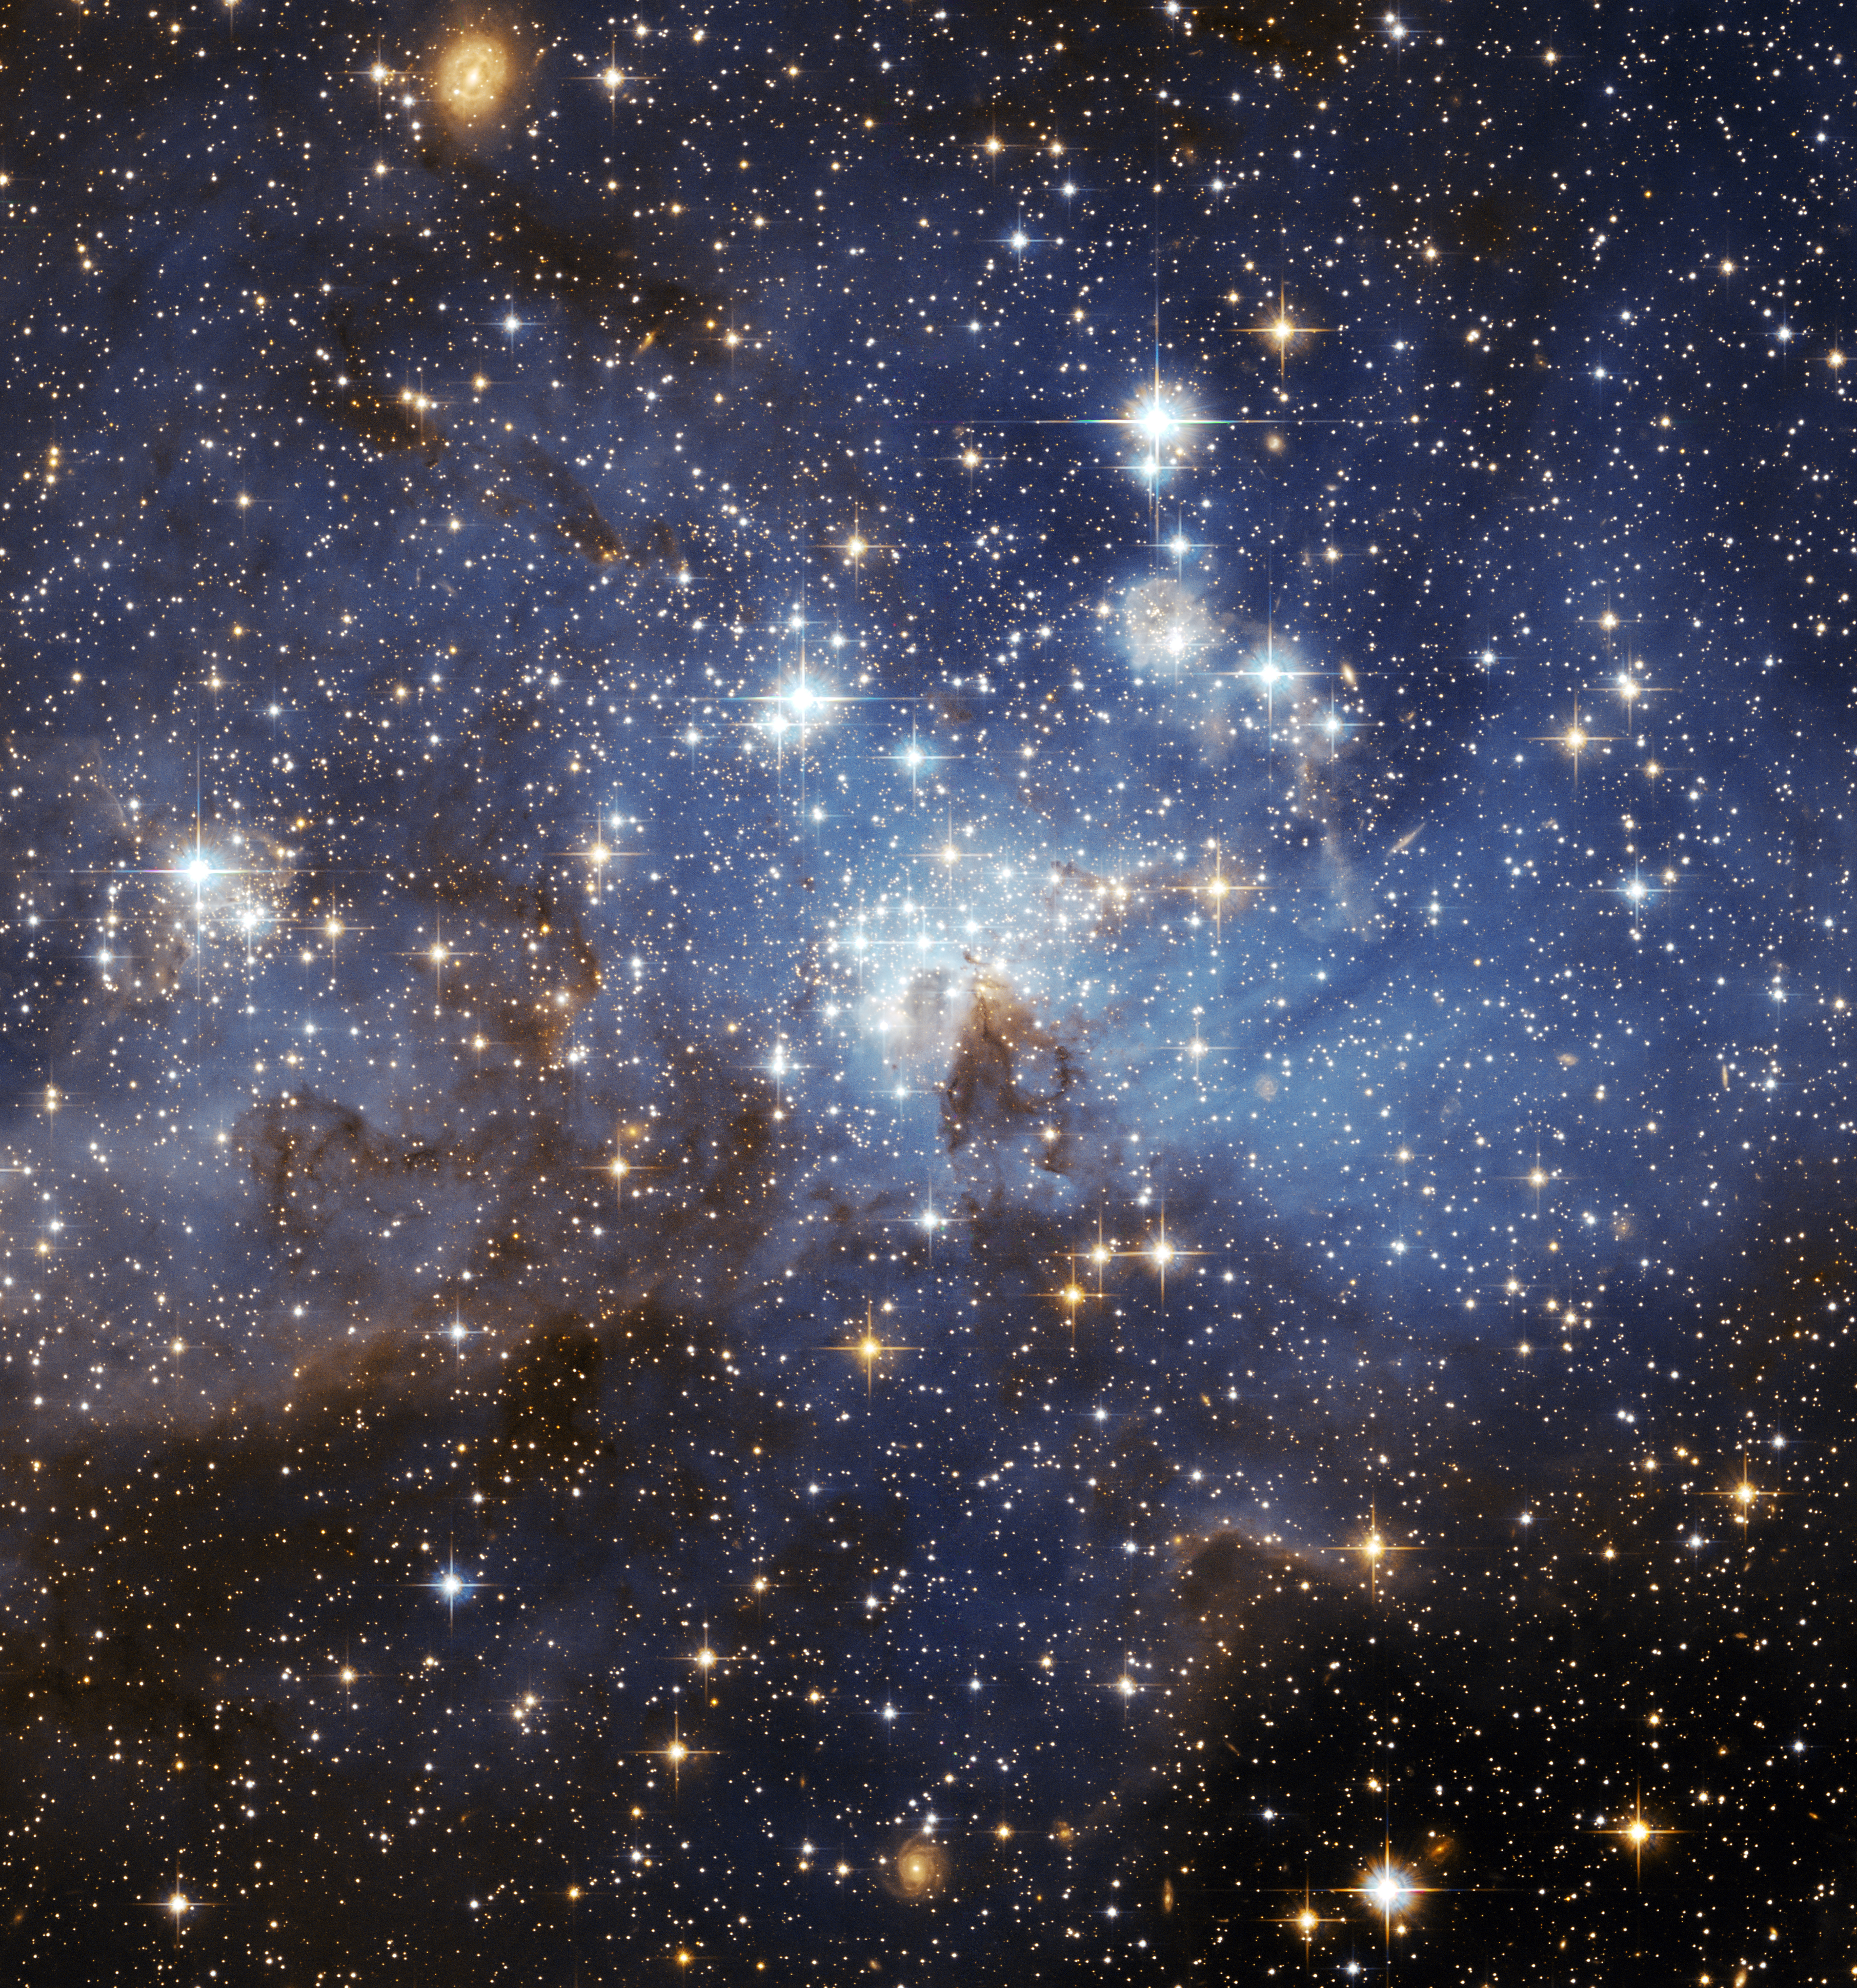
\includegraphics[height=1.75\invitationheight]{cover.jpg}};
		\covertext[invitation text] (uitnodiging) at ($(invitation.north)!.0!(invitation.south)$) {\invtextwidth}%
			{\centering Uitnodiging}@\Huge;
		\covertext[invitation text] (bijwonen) at (uitnodiging.south) {\invtextwidth}%
			{\nohyphenation\Centering voor het bijwonen van de openbare verdediging van mijn proefschrift}@\large;
		\covertext[invitation text] (invitation title) at ($(bijwonen.south)+(0,-2.5mm)$) {\invtextwidth}%
			{\nohyphenation\Centering\thesistitle}@\Large;
		\covertext[invitation text] (invitation subtitle) at ($(invitation title.south)+(0,1mm)$) {\invtextwidth}%
			{\nohyphenation\Centering\thesissubtitle}@{\large\itshape};
		\covertext[invitation text] (invitation date) at ($(invitation subtitle.south)+(0,-2.5mm)$) {\invtextwidth}%
			{\nohyphenation\Centering%
				op \mbox{\displaydate{thesis}} om 14.30~uur %
				in de Berkhoff~zaal van het gebouw de~Waaier van de Universiteit~Twente.
				Aansluitend is er een receptie.%
			}@\large;
		\covertext[invitation text] (invitation author) at (invitation date.south) {\invtextwidth}%
			{\nohyphenation\Centering%
				Jochem Rutgers\\\vspace{.75ex}%
				Park de Kotten 102\\%
				7522 EE {} Enschede\\%
				06\,-\,1292\,5775\\%
				\href{mailto:j.h.rutgers@alumnus.utwente.nl}{j.h.rutgers@alumnus.utwente.nl}%
				}@\large;
		\covertext[invitation text] (author contact) at ($(invitation.north)!.9!(invitation.south)$) {\invtextwidth}%
			{\nohyphenation\Centering}@\normalsize;
%		\node[text back,fit={($(invitation.north)+(0,\marginwidth)$) (author contact)}] {};
		\fill [black,path fading=invitation fade] ($(invitation.north west)+(-\bleedwidth,\bleedwidth)$) rectangle ($(invitation.north east)!.85!(invitation.south east)+(\bleedwidth,0)$);
	\end{scope}
\end{invitation}

\end{document}
